%%%%%%%%%%%%%%%%%%%%%%%%%%%%%%%%%%%%%%%%%%%%%%%%%%%%%%%%%%%%%%%%%%%%%%%%%%%
%%%                                                                     %%%
%%%   LaTeX template voor het verslag van P&O: Computerwetenschappen.   %%%
%%%                                                                     %%%
%%%   Opties:                                                           %%%
%%%     tt      Tussentijdsverslag                                      %%%
%%%     eind    Eindverslag                                             %%%
%%%                                                                     %%%
%%%   4 november 2013                                                   %%%
%%%   Versie 1.1                                                        %%%
%%%                                                                     %%%
%%%%%%%%%%%%%%%%%%%%%%%%%%%%%%%%%%%%%%%%%%%%%%%%%%%%%%%%%%%%%%%%%%%%%%%%%%%

\documentclass[tt]{penoverslag}

%%% PACKAGES %%%
\usepackage{graphicx}
\setlength\parindent{0pt}

\begin{document}

% == TITELPAGINA == %
\team{Indigo} % teamkleur
\members{\\
        Wander Bavin\\
        Vince Goossens\\
        Dimitri Jonckers\\
        Sunil Tandan\\
		Wout Vekemans\\} % teamleden
\maketitlepage


% == SAMENVATTING == %
\begin{abstract}

\end{abstract}


% == INHOUDSOPGAVE == %
\tableofcontents\newpage


% == INLEIDING == %
\section{Inleiding}
Het doel van deze opdracht is een autonome zeppelin te ontwikkelen. De zeppelin wordt aangestuurd door een Raspberry Pi. Via QR-codes kunnen instructies gegeven worden, zoals ``stijg 50cm'' of ``draai 45   graden''. De gebruiker kan via een GUI op een client-pc zelf de pijltjestoetsen gebruiken om de zeppelin aan te sturen of gegevens bekijken over de toestand van de zeppelin (bijvoorbeeld de huidige hoogte).

\paragraph{Fysisch ontwerp}
~\\ 
De zeppelin bestaat uit een houten frame waaraan 2 grote ronde heliumballonnen vastgemaakt zijn. Aan het frame is een afstandssensor gekoppeld die naar onderen is gericht. Verder is er een camera naar beneden gericht. Zowel de camera alsook de afstandssensor zijn verbonden met de Raspberry Pi die in het frame zit ingebed. Het geheel bevat drie propellers: twee voor zijwaartse bewegingen en \'{e}\'{e}n voor opwaartse bewegingen.


\paragraph{Software ontwerp}
~\\
Natuurlijk moet de zeppelin aangestuurd worden via de software. Dit is onderverdeeld in 3 grote delen: de GUI, de communicatie tussen GUI en Raspberry Pi en de interne programmatie op de Pi (Zie figuur \ref{schema}). De software zal volledig worden geprogrammeerd in Java. 
De communicatie tussen GUI en de Raspberry Pi gebeurt via sockets. Hierbij worden objecten uitgewisseld tussen de client en de server (de Pi), die commando's doorgeven aan de zeppelin of de status doorgeven aan de gebruiker. De interne programmatie op de Pi moet op basis van gegevens van zijn sensoren en instructies van QR-codes (en commando's van de gebruiker) de motoren aansturen. 

\begin{figure}[ht!]
\centering
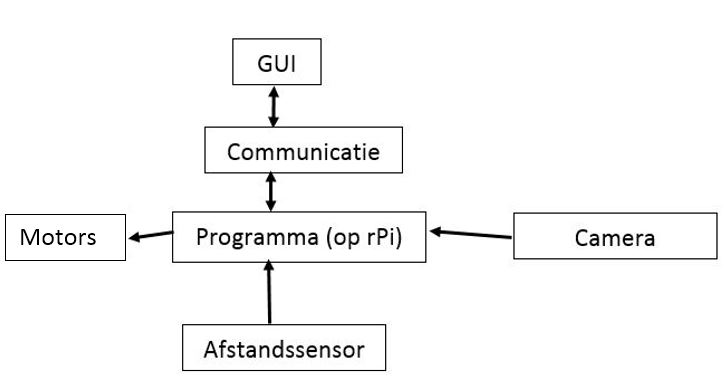
\includegraphics[height=55mm]{Schema.jpg}
\caption{Architectuur}
\label{schema}
\end{figure}


% == Beschrijving materiaal en bouw zeppelin == %
\section{Beschrijving materiaal en bouw zeppelin}
Alle onderdelen van de zeppelin zullen gemonteerd worden op een frame. Hierop worden 3 propellers bevestigd. Twee hiervan dienen om naar links en rechts te draaien. Om vooruit te bewegen worden deze samen geactiveerd met dezelfde kracht. De derde propeller dient om de zeppelin te laten stijgen, dus is naar beneden gericht. ~\\

Om het geheel in de lucht te houden, hangen er 2 ballonnen tegen de bovenkant van het frame. Deze hebben een diameter van ongeveer 90 centimeter en bevatten helium. \\
\\
De zeppelin wordt aangestuurd door een Raspberry Pi model A (zie Figuur \ref{Pi}). Deze heeft volgende specificaties: 
\begin{itemize}
	\item \emph{Processor:} 700MHz ARM
	\item \emph{Geheugen:} 256MB 
	\item \emph{Poorten:} 1 USB 2.0, HDMI, audio out, RCA video
	\item \emph{Voeding:} Micro USB
	\item GPIO-pinnen om de hardware aan te sturen
\end{itemize}

In de Raspberry Pi zit een SD-kaart van 4 GB. Op de USB-poort is een USB hub aangesloten, zodat het mogelijk is meerdere onderdelen aan te sluiten. Deze gebruiken we voor een toetsenbord, muis en WiFi dongle. \\

Verder zijn er nog 2 devices waarvan de zeppelin gebruik maakt:
\begin{itemize}
	\item De camera laat toe foto's te nemen met een maximum resolutie van 5 MP. Hiermee kunnen we onder andere beelden maken van QR-codes. Daarnaast kan de camera video's maken met resoluties tot 1080p. 
	\item De afstandssensor kan worden gebruikt om de afstand te meten tussen de zeppelin en de grond of muur. Het maximale bereik is 4m en het minimale bereik is 2cm.\\
\end{itemize}

Om er zeker van te kunnen zijn dat het aansturen van de zeppelin correct gebeurt, is het nodig dat de componenten getest worden. In de volgende secties volgt hierover meer informatie.\\

\begin{figure}[ht!]
\centering
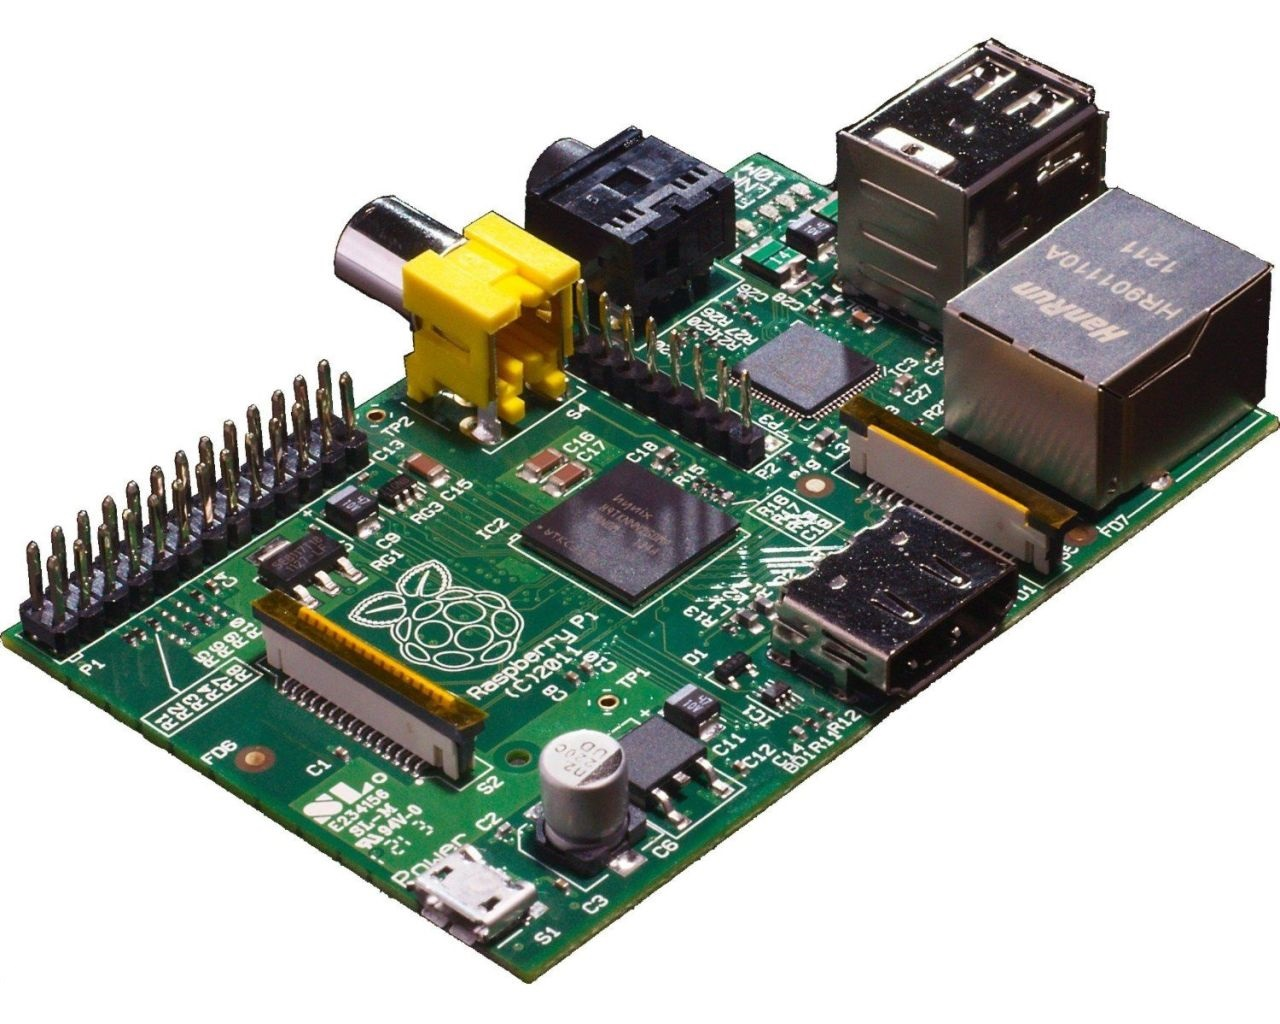
\includegraphics[height=30mm]{raspb.jpg}
\caption{Raspberry Pi}
\label{Pi}
\end{figure}



% == Testen == %
\section{Testen}
\subsection{Afstandssensor}

In deze sectie gaan we dieper in op de testen die we gedaan hebben naar de nauwkeurigheid en snelheid van de afstandssensor.

\paragraph{Opstelling} ~\\ 
Benodigdheden:
\begin{itemize}
	\item RaspberryPi met afstandssensor
	\item houten scherm
	\item meetlat
\end{itemize}
Deze componenten worden in deze opstelling geplaatst : zie figuur \ref{opstelling}
\begin{figure}[ht!]%
\centering
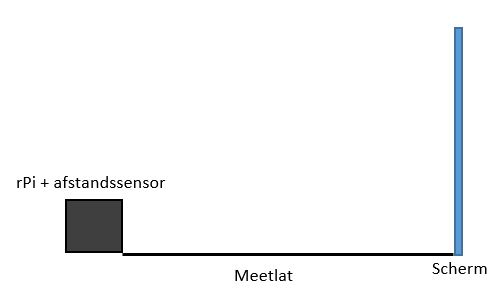
\includegraphics[scale=0.6]{opstelling.jpg}%
\caption{testopsteling}%
\label{opstelling}%
\end{figure}

\paragraph{Verloop} ~\\ 
De test bestaat uit het meten van 11 verschillende afstanden (10, 20, 30, 60, 90, 100, 110, 120, 130, 140 en 150 cm). Deze zijn zo gekozen om meer kennis te hebben over kleine afstanden en over de verwachte vlieghoogte. Deze afstanden worden elk 500 keer gemeten, om de 60 ms. Deze waarden zijn zo gekozen, om toch voldoende nauwkeurigheid te hebben, veronderstellende dat er uitschieters zouden zijn. We focussen ons op nauwkeurigheid en snelheid.

\paragraph{Gegevens en verwerking} ~\\ 
Het uitvoeren van de testen nam per afstand gemiddeld 32 seconden in beslag. Omdat dit tijdens het opereren van de zeppelin onhaalbaar is, hebben we besloten om het interval te verlagen. Zo kunnen de metingen sneller gebeuren. Hiervoor hebben we een extra test uitgevoerd op een hoogte van 170cm. Het blijkt dat we het interval tussen metingen kunnen verlagen tot 40 ms. Bij lagere waardes gaan signalen door elkaar lopen en zo de meting verstoren. \\

Omdat 500 metingen nog steeds 20 seconden duren, hebben we het aantal verlaagd. We hebben d.m.v. rolling median de mediaan berekend van 10 en 20 opeenvolgende gegevens. Minder dan 10 is niet nauwkeurig genoeg, en voor meer dan 20 samples is de registratietijd te hoog. Uit deze gegevens hebben we om een aantal redenen besloten om een window van 10 samples te nemen.  Ten eerste is er de nauwkeurigheid als de zeppelin stijgt/daalt. Het hoogteverschil tussen sample 1 en 10 is immers kleiner dan dat tussen 1 en 20. Ten tweede is er de snelheid. Het spreekt voor zich dat het registreren van 10 samples minder lang duurt dan 20 samples. Tenslotte is er ook het minieme verschil tussen de gemiddelde mediaan bij 10 en 20 metingen. Minder metingen zorgen dus voor een even grote nauwkeurigheid. 

Een nadeel is wel dat de standaardafwijking van de medianen bij een breedte van 10 samples gemiddeld 0.2 cm groter is dan bij 20 samples. Dit weegt echter niet op tegen de winst aan snelheid en nauwkeurigheid.\\ 

Voor de meetgegevens: zie onderstaande tabel. \\

\begin{tabular}{r||r|r|r|r|r|r|r|r|r|r|r}
\textbf{Afstand} & 10 & 20 & 30 & 60 & 90 & 100 & 110 & 120 & 130 & 140 & 150 \\
\hline \hline 
$\mu$ (med.) (10) & 10.8 & 20.5 & 30.8 & 58.0 & 88.3 & 98.7 & 108.5 & 117.3 & 127.74 & 137.0 & 147.10 \\
$\mu$ (med.) (20) & 10.8 & 20.7 & 30.7 & 58.0 & 88.3 & 98.7 & 108.5 & 117.3 & 127.7 & 137.0 & 147.1 \\
$\sigma$ (med.) (10) & 0.21 & 0.52 & 0.82 & 0.55 & 0.70 & 0.72 & 0.68 & 0.94 & 0.58 & 0.60 & 0.69 \\
$\sigma$ (med.) (20)& 0.09 & 0.33 & 0.71 & 0.41 & 0.59 & 0.56 & 0.47 & 0.54 & 0.43 & 0.37 & 0.49 \\
\end{tabular}

\paragraph{Conclusie} ~\\ 
De afstandsmeter meet het meest nauwkeurig bij kleine afstanden, bij grotere afstanden (meer dan 60 cm) liggen de meetresultaten gemiddeld iets onder de opgelegde afstand. Relatief gezien blijft de fout nog klein en kunnen we deze afwijking in het vervolg incalculeren bij het bepalen van de meetwaarden. De afstandssensor geeft telkens de mediaan van 10 gegevens door volgens het principe van de “rolling median”-techniek. Tien gegevens zorgen voor voldoende nauwkeurigheid, maar hebben ook het aspect dat de mediaanberekeningen snel genoeg gebeuren. Tevens is dit bij een hoogteverandering accurater. Deze methode boet wel in op de standaardafwijking. De gegevens wijken dus meer uit, maar dit weegt niet op tegen de voorgenoemde pluspunten. Om de afstandsregistratie nog sneller te laten verlopen, meet de afstandsmeter om de 10 ms. Een vertraging van 32 seconden is niet acceptabel.

\subsection{Camera}

\textbf{Deze is nog niet uitgevoerd.} \\

Het testen van de camera lijkt op het eerste zicht eenvoudig, maar er komt veel meer bij kijken dan enkel foto's nemen. Er moet rekening gehouden worden met lichtintensiteit, responstijd van de camera, positie van de QR-code op de foto, \ldots \\

De lichtintensiteit wordt getest in een kamer met controleerbare lichtbron (d.m.v. lichtschakelaar, verduistering). Er wordt getest hoe licht het moet zijn in de kamer opdat de QR-code in de foto nog herkend wordt door het programma. \\

We hebben al kleine testen uitgevoerd waarin de QR-code lichtjes gedraaid was (invalshoek), en er was geen probleem om ze te lezen. Omdat de QR-code altijd recht onder de zeppelin zal staan, gaan we dit niet verder testen. \\

De responstijd (tijd tot herkennen QR-code) wordt getest door in verschillende omstandigheden een code te fotograferen. Een simpel printcommando in Java vertelt ons hoe lang het verwerken duurt. Hiervoor wordt de interne klok van de computer gebruikt. Om een globaal beeld te krijgen van de responstijd wordt een gemiddelde berekend van deze gegevens. We verwachten dat op grotere hoogtes (grotere afstand tot de code) we een afbeelding moeten nemen in hogere resolutie, waardoor de verwerkingstijd langer zal zijn. \\

Om te bepalen tot op welke afstand de camera foto's kan maken die herkend kunnen worden, is er een simpele test: de camera fotografeert een QR-code vanop verschillende afstanden. 
De positie van de QR-code in de foto is een cruciaal element. De codes bevatten commando’s die relatief ten opzichte van de huidige positie moeten worden uitgevoerd. Kleine afwijkingen van de positie van de code tot het midden van de foto zijn onvermijdelijk en zullen zich voortplanten tijdens het verderzetten van het parcours. Dit heeft echter meer betrekking tot het testen en calibreren van de motoren (zie verder). \\


\subsection{Motoren}
\textbf{Deze is nog niet uitgevoerd.} \\

\paragraph{Zijwaartse bewegingen} ~\\ 
Om de zijwaartse bewegingen te testen, gaan we kijken hoe lang we de motor moeten aanzetten om een hoek van 10$^\circ$ , 20$^\circ$, 30$^\circ$, \ldots uit te voeren. We zullen deze testen uitvoeren op hoeken naar links. Hiervoor zetten we de linkermotor op volle kracht achteruit en de rechtermotor op volle kracht vooruit. \\

Om dit te testen, gaan we de zeppelin moeten positioneren boven een soort 'roos': een cirkel waarop de graden staan aangeduid. Aan de hand van foto's van de naar onder gerichte camera, kunnen we dan manueel aflezen hoe ver de zeppelin gedraaid is. \\

Indien we deze gegevens voor hoeken van 10 tot 180 graden hebben, kunnen we deze plotten. Hier verwachten we een lineair patroon te zien vanaf een bepaalde hoek. Dit gaat namelijk zijn bij de hoek waarbij de maximale kracht van de motor bereikt is. Het lineair patroon gaat doorbroken worden wanneer de gevraagde hoek bijna is bereikt. \\

Wanneer we deze functie gevonden hebben, zijn enkel de volgende gegevens nodig:
\begin{itemize}
	\item data voor voldoende hoeken kleiner dan de kritieke hoek waarbij het maximumvermogen van de motor wordt bereikt
	\item de lineaire functie
	\item hoe lang het duurt om uit te bollen
\end{itemize}
Voor kleine hoeken kunnen we dan een soort van tabel raadplegen, voor hoeken groter dan de kritieke hoek gebruiken we de lineaire functie. \\

Als laatste moeten we controleren dat deze gegevens hetzelfde zijn voor bewegingen naar de rechterkant.  Dit doen we door dezelfde gegevens voor een aantal hoeken toe te passen. \\

\paragraph{Voorwaartse bewegingen} ~\\ 
Om voorwaartse bewegingen uit te voeren, zetten we zowel linker als rechter motor aan. Uit de testen die we gedaan hebben bij zijwaartse bewegingen, weten we of de 2 motoren hetzelfde afgesteld zijn. Indien ze niet perfect afgesteld zijn, zullen we moeten testen hoe vaak we tijdelijk de krachtigste motor moeten uitschakelen om een zo perfect mogelijke rechte baan te bekomen. \\

Het testen van de voorwaartse beweging gaat heel gelijkaardig zijn aan het testen van de zijwaartse bewegingen.  De zeppelin beweegt boven een liniaal.  Aan de hand van foto's van de camera kunnen we zien hoever hij van de rechte lijn bewogen is en hoever hij geraakt is. We gaan opnieuw kunnen afleiden na hoeveel tijd de zeppelin zijn maximum vermogen bereikt. Zo gaan we opnieuw een formule opstellen die we dan gebruiken om te bepalen hoe lang we de motoren moeten laten draaien om een bepaalde afstand af te leggen. \\

\paragraph{Verticale bewegingen} ~\\ 
We gaan allereerst op zoek naar de juiste pwm waarde waarbij de zeppelin op dezelfde hoogte blijft zweven ('zweef-pwm').  Dit gebeurt wanneer de stuwkracht gelijk is aan de gravitatiekracht.  Vervolgens gaan we uitzoeken hoeveel centimeter de zeppelin nog extra stijgt wanneer we overgaan van maximale pwm naar zweef-pwm.\\



% == ALGORITMES == %
\section{Algoritmes}



% == SOFTWARE == %
\section{Software}
Zoals reeds vermeld, zal de software volledig in Java geschreven zijn. Deze keuze hebben we gemaakt omdat we al veel ervaring hebben met het schrijven van Java-programma's. Python was een andere mogelijke keuze. Er is veel voorbeeldcode in Python te vinden voor de Raspberry Pi, maar we hebben voor de functies die wij nodig hebben voldoende kennis en referenties in Java gevonden. Het leren van een extra taal zou erg tijdrovend in verhouding met de voordelen die het brengt. \\

Om de software te schrijven, gaan we op de laptop gebruik maken van de Eclipse IDE. We maken ook gebruik van de Netbeans IDE. Deze is door de visuele interface veel gebruikvriendelijker om de GUI te ontwerpen. Hierdoor moeten we ons niet bezig houden met alle code voor de lay-out handmatig te schrijven. Voor het aansturen van de GPIO-pinnen gebruiken we Pi4J\footnote{www.pi4j.com}.\\

Op een client-pc kan de GUI (zie figuur \ref{GUI}) worden gestart. Hier kan de gebruiker informatie aflezen over de toestand van de zeppelin (bijvoorbeeld de hoogte, commando's die hij aan het uitvoeren is) en afbeeldingen van de camera bekijken. Verder kan de gebruiker de zeppelin aansturen via de pijltjestoetsen. \\

De communicatie tussen de GUI (client) en de Raspberry Pi (server) gebeurt via sockets. Sockets zijn een eenvoudige en universele manier om data over een netwerk te sturen. Ze zijn te vergelijken met een deur waarlangs objecten van klassen uitgewisseld worden. Deze stellen bijvoorbeeld commando's van de gebruiker voor of de status van de zeppelin die aan de GUI wordt doorgegeven. Concreet opent de server een socket op poort 6789 (de eerste 1024 poorten zijn gereserveerd voor services zoals http en ftp, we hebben een willekeurige poort hierachter gekozen). Hierop kan 1 client verbinden. Het zou mogelijk zijn meerdere clients toegang te geven, maar om conflicten (met pijltjestoetsen) te vermijden en om bandbreedte te besparen (bij het doorsturen van afbeeldingen), ondersteunt de server maar 1 client.  \\

Om meerdere taken tegelijk te kunnen uitvoeren, maken we gebruik van threads. Zo kan de zeppelin tegelijk foto's nemen en de afstand tot de grond meten. Later zal worden beslist hoeveel gelijklopende threads er gebruikt worden. \\

Alle software behalve de GUI draait op de Raspberry Pi, omdat die autonoom moet kunnen werken. Hier worden beslissingen genomen op basis van QR-codes, die uit afbeeldingen komen die de camera op geregelde tijdstippen neemt. Elke opname van de camera wordt naar de GUI doorgestuurd. Het verwerken van de beelden zal gebeuren op de Raspberry Pi. Logisch gezien is het weergeven van de status van de zeppelin echter geen taak van de Pi zelf. Daarom draait de GUI op de client. Daarnaast wordt door deze keuze de CPU van de Pi minder zwaar belast. \\

De hoogte zal op bepaalde momenten opgemeten worden. Om een zo accuraat mogelijke waarde te krijgen, wordt de mediaan genomen van een aantal opeenvolgende meetresultaten. De hoogte wordt, net zoals de foto's, doorgestuurd naar de GUI. Om de afbeelding te doorzoeken op QR-codes, maken we gebruiken van ZXing\footnote{http://code.google.com/p/zxing/} (Zebra Crossing). Dit is een bekend project voor het inlezen van QR-codes dat oorspronkelijk in Java geschreven is. \\

\begin{figure}[ht!]
\centering
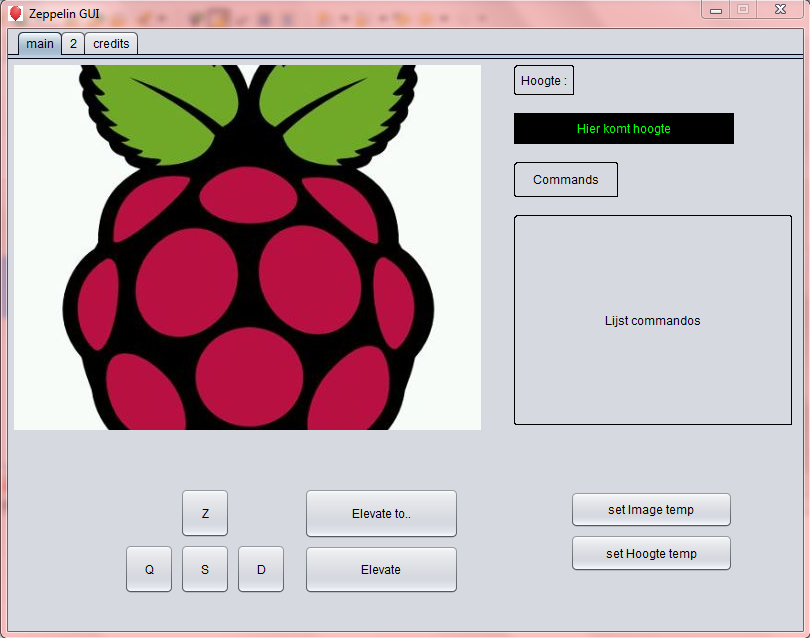
\includegraphics[height=40mm]{GUI.png}
\caption{GUI}
\label{GUI}
\end{figure}


% == GUI == %
\section{GUI}





% == BESLUIT == %
\section{Besluit}



% == REFERENTIES == %
\bibliographystyle{siam}
\bibliography{references.bib}


% == APPENDICES == %
\newpage\makeappendix

\section{Beschrijving van het proces}
\begin{itemize}
\item Welke moeilijkheden heb je ondervonden tijdens de uitwerking?
\item Welke lessen heb je getrokken uit de manier waarop je het project hebt aangepakt?
\item Hoe verliep het werken in team? Op welke manier werd de teamco\"ordinatie en planning aangepakt?
\end{itemize}


\section{Beschrijving van de werkverdeling}
\begin{itemize}
\item Geef voor elk van de groepsleden aan aan welke delen ze hebben meegewerkt en welke andere taken ze op zich hebben genomen.
\item Rapporteer in tabelvorm hoeveel uur elk groepslid elke week aan het project gewerkt heeft, zowel tijdens als buiten de begeleide sessies. Geef ook totalen per groepslid voor het volledige semester.
\end{itemize}


\section{Kritisch analyse}
\begin{itemize}
\item Maak een analyse van de sterke en zwakke punten van het project. Welke punten zijn vatbaar voor verbetering. Wat zou je, met je huidige kennis, anders aangepakt hebben?
\end{itemize}


\end{document}
